\chapter{2重平面振子}

ランダウ、リフシッツ「力学」p13問題1(図1)

\section{モデルの定式化}

%\begin{comment}
\begin{figure}[htbp]
  \begin{minipage}[b]{0.45\linewidth}
    \centering
    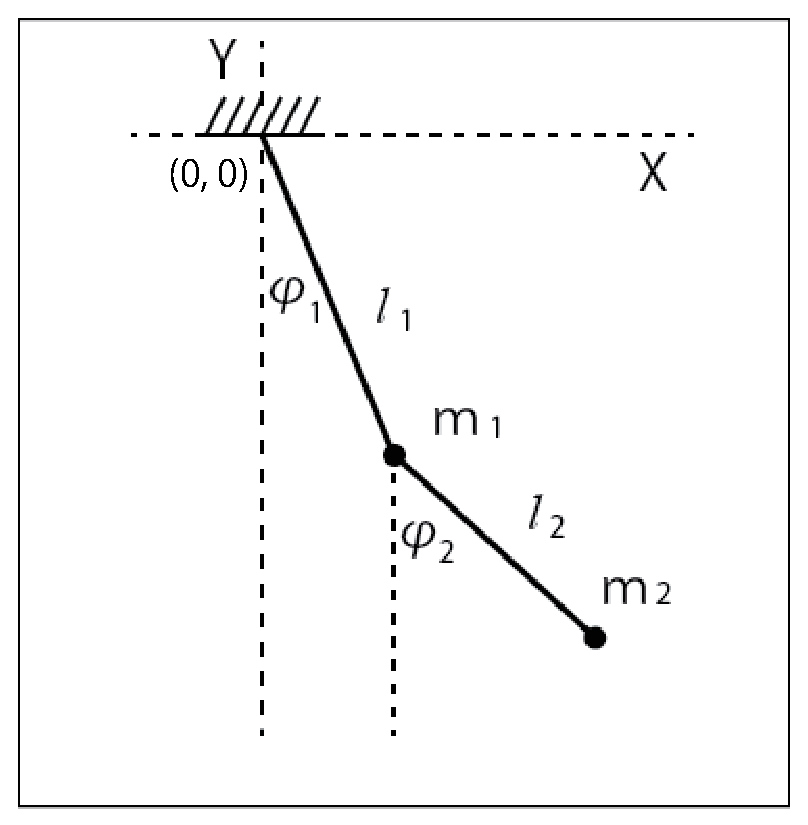
\includegraphics[keepaspectratio, scale=0.5]{eps/double.eps}
    \caption{2重平面振子}
  \end{minipage}
  %\begin{minipage}[b]{0.45\linewidth}
    %\centering
    %\includegraphics[keepaspectratio, scale=0.35]{p13-2.eps}
    %\caption{p13-2}
  %\end{minipage}
\end{figure}
%\end{comment}

棒$l_1$及び$l_2$が鉛直となす角を$\varphi_1,\varphi_2$とする.座標原点を支点におくことにすると, 質点の座標はそれぞれ

\[
(l_1\sin\varphi_1, -l_1\cos\varphi_1), \qquad (l_1\sin\varphi_1+l_2\sin\varphi_2, -l_1\cos\varphi_1-l_2\cos\varphi_2)
\]

質点$m_1$に対する運動エネルギー$T_1$,及びポテンシャル・エネルギー$U_1$は,

\[
\displaystyle T_1=\frac{1}{2}m_1(l_1\dot{\varphi_1})^2\quad,\qquad U_1=-m_1gl_1\cos\varphi_1
\]

($\displaystyle T_1=\frac{1}{2}m_1(\dot{x_1}^2+\dot{y_1}^2)$を計算しても,同じ結果になる.)\\

一方質点$m_2$について, そのデカルト座標$(x_2,y_2)$から,
\begin{align*}
x_2&=l_1\sin\varphi_1+l_2\sin\varphi_2\quad,\quad y_2=-(l_1\cos\varphi_1+l_2\cos\varphi_2)\\
\dot{x_2}&=l_1\dot{\varphi_1}\cos\varphi_1+l_2\dot{\varphi_2}\cos\varphi_2\quad,\quad\dot{y}_2=l_1\dot{\varphi_1}\sin\varphi_1+l_2\dot{\varphi_2}\sin\varphi_1\\
\dot{x}_2^2&=l_1^2\dot{\varphi_1}^2\cos^2\varphi_1+2l_1l_2\dot{\varphi_1}\dot{\varphi_2}\cos\varphi_1\cos\varphi_2+l_2^2\dot{\varphi_2}^2\cos^2\varphi_2\quad,\\
\dot{y}_2^2&=l_1^2\dot{\varphi_1}^2\sin^2\varphi_1+2l_1l_2\dot{\varphi_1}\dot{\varphi_2}\sin\varphi_1\sin\varphi_2+l_2^2\dot{\varphi_2}^2\sin^2\varphi_2
\end{align*}

運動エネルギーとポテンシャル・エネルギーは,\\
$\cos(\alpha-\beta)=\cos\alpha\cos\beta+\sin\alpha\sin\beta$,また $\sin^2\alpha+\cos^2\alpha=1$だから

\begin{align*}
\displaystyle T_2&=\frac{1}{2}m_2(\dot{x_2}^2+\dot{y_2}^2)=\frac{m_2}{2}\left(l_1^2\dot{\varphi_1}^2+l_2^2\dot{\varphi_2}^2+2l_1l_2\cos(\varphi_1-\varphi_2)\dot{\varphi_1}\dot{\varphi_2}\right)\\\\
U_2&=-m_2gl_1\cos\varphi_1-m_2gl_2\cos\varphi_2
\end{align*}

従って,Lagrangian$L=T_1+T_2-U_1-U_2$は,

\begin{align*}
L&=\displaystyle\frac{m_1+m_2}{2}l_1^2\dot{\varphi_1}^2+\frac{m_2}{2}l_2^2\dot{\varphi_2}^2+m_2l_1l_2\dot{\varphi_1}\dot{\varphi_2}\cos(\varphi_1-\varphi_2)\\\\
&\quad+(m_1+m_2)gl_1\cos\varphi_1+m_2gl_2\cos\varphi_2
\end{align*}

になる. 

\begin{align*}
\displaystyle\frac{\partial L}{\partial\varphi_1}&=-m_2l_1l_2\sin(\varphi_1-\varphi_2)\dot{\varphi_1}\dot{\varphi_2}-(m_1+m_2)gl_1\sin\varphi_1\quad,\\\\
\displaystyle\frac{\partial L}{\partial\dot{\varphi_1}}&=(m_1+m_2)l_1^2\dot{\varphi_1}+m_2l_1l_2\cos(\varphi_1-\varphi_2)\dot{\varphi_2}\quad,\\\\
\displaystyle\frac{\partial L}{\partial\varphi_2}&=m_2l_1l_2\sin(\varphi_1-\varphi_2)\dot{\varphi_1}\dot{\varphi_2}-m_2gl_2\sin\varphi_2\quad,\\\\
\displaystyle\frac{\partial L}{\partial\dot{\varphi_2}}&=m_2l_2^2\dot{\varphi_2}+m_2l_1l_2\cos(\varphi_1-\varphi_2)\dot{\varphi_1}
\end{align*}

より, Euler-Lagrange eq.

\[
\displaystyle \frac{\mathrm{d}}{\mathrm{d}t}\frac{\partial L}{\partial \dot{\varphi_i}}-\frac{\partial L}{\partial \varphi_i}=0
\]

は,

\begin{align*}
(m_1+m_2)l_1^2\ddot{\varphi_1}+m_2l_1l_2\cos(\varphi_1-\varphi_2)\ddot{\varphi_2}+m_2l_1l_2\sin(\varphi_1-\varphi_2)\dot{\varphi_1}\dot{\varphi_2}+(m_1+m_2)gl_1\sin\varphi_1&=0,\\\\
m_2l_2^2\ddot{\varphi_2}+m_2l_1l_2\cos(\varphi_1-\varphi_2)\ddot{\varphi_1}-m_2l_1l_2\sin(\varphi_1-\varphi_2)\dot{\varphi_1}\dot{\varphi_2}+m_2gl_2\sin\varphi_2&=0
\end{align*}

\section{Pythonによる模擬実験}

連立の常微分方程式にして,関数odeを定義する.

\begin{align*}
\displaystyle\frac{\mathrm{d}\varphi_1}{\mathrm{d}t}&=\dot{\varphi_1}\\\\
\displaystyle\frac{\mathrm{d}\varphi_2}{\mathrm{d}t}&=\dot{\varphi_2}\\\\
\displaystyle\frac{\mathrm{d}\dot{\varphi_1}}{\mathrm{d}t}&=\frac{Mg\sin\varphi_1+m_2\sin H(l_1\cos H+l_2)\dot{\varphi_1}\dot{\varphi_2}-m_2g\cos H\sin\varphi_2}{-\left(Ml_1-m_2l_1\cos^2H\right)}\\\\
\displaystyle\frac{\mathrm{d}\dot{\varphi_2}}{\mathrm{d}t}&=\frac{Mg\cos H\sin\varphi_1+\sin H(Ml_1+m_2l_2\cos H)\dot{\varphi_1}\dot{\varphi_2}-Mg\sin\varphi_2}{Ml_2-m_2l_2\cos^2H}
\end{align*}

ここで, $H=\varphi_1-\varphi_2 ,\quad M=m_1+m_2$である.

単振子との違いは質点が2個あるので,関数odeの戻り値は,単振子のときに$\left[\varphi, \dot{\varphi}\right]$としていたのを,$\left[\varphi_1, \dot{\varphi_1}, \varphi_2, \dot{\varphi_2}\right]$とする.

積分は,scipy.integrateのodeintを,アニメーションは,matplotlib.animationのFuncAnimationを使う.

\lstset{escapechar=@,style=custompy}
\lstinputlisting[caption=2重平面振子,label=pythonProgram2]{py/double.py}
